\begin{question}
Using the \emph{probability integral transform} transform a Gumbel distribution into a Gaussian. Plot also all the distributions involved in the transformation.
\end{question}

\cprotEnv\begin{solution}
\begin{ipython}
from scipy.stats import gumbel_l, norm
from matplotlib import pyplot as plt

gumbel = gumbel_l()
xg = gumbel.rvs(100000)
xu = gumbel.cdf(xg)
xn = norm.ppf(xu)

sub1 = plt.subplot(1, 3, 1)
sub1.hist(xg, 50)
sub1.grid(True)
sub1.set_xlabel("$x_{gumbel}$")
sub2 = plt.subplot(1, 3, 2)
sub2.hist(xu, 50)
sub2.grid(True)
sub2.set_xlabel("$x_{uniform}$")
sub3 = plt.subplot(1, 3, 3)
sub3.hist(xn, 50)
sub3.grid(True)
sub3.set_xlabel("$x_{normal}$")
plt.show()
\end{ipython}

\begin{figure}[htbp]
\begin{center}
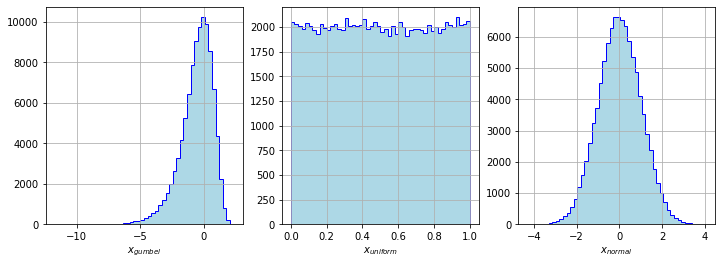
\includegraphics[width=0.9\linewidth]{figures/ex_gumbel_to_gauss.png}
\end{center}
\end{figure}
\end{solution}

\begin{question}
Without using the corresponding \texttt{rvs()} method try to generate 10 random numbers distributed as Beta distribution (parameters \texttt{a=3} and \texttt{b=10}).

\noindent\textbf{Hint:} starts with generating uniformly distributed random numbers.
\end{question}	

\cprotEnv\begin{solution}
\begin{ipython}
from scipy.stats import beta, uniform

x = uniform.rvs(size=10)
b = beta(a=3, b=10)
x_b = b.ppf(x)

print (x_b)
\end{ipython}
\begin{ioutput}
[0.29190237 0.45669406 0.10336582 0.5403107 0.08305872 0.32425694
0.43902811 0.11820592 0.28659784 0.22316621]
\end{ioutput}
\end{solution}

\begin{question}
Consider two companies whose default probabilities as a function of time are modeled according to a lognormal distribution with $\sigma =0.5$ (\texttt{scipy.stats.lognorm(0.5)}). Compare the joint 2D distributions in case of no correlation and with a Gaussian correlation of 0.8.

\noindent\textbf{Hint:} to plot the joint distribution use \texttt{matplotlib} function \texttt{hist2d(x1, x2, range=[[x1min, x1max], [xmin, x2max]], bins=(50, 50)) }.
\end{question}

\cprotEnv\begin{solution}
\begin{ipython}
from scipy.stats import lognorm, multivariate_normal, norm
import numpy

numpy.random.seed(1)
samples = 1000000
l1_uncorr = lognorm(0.5).rvs(size=samples)
l2_uncorr = lognorm(0.5).rvs(size=samples)
mvnorm = multivariate_normal(mean = (0, 0), 
                             cov = [[1, 0.8],
                                    [0.8, 1]])
x = mvnorm.rvs(size=samples)
x_corr = norm.cdf(x)
l1_corr = lognorm(0.5).ppf(x_corr[:, 0])
l2_corr = lognorm(0.5).ppf(
x_corr[:, 1])
plt.figure(figsize=(12, 4))
sub1 = plt.subplot(1, 2, 1)
sub1.hist2d(l1_uncorr, l2_uncorr, range=[[0, 2], [0, 2]], bins=(100, 100))
sub2 = plt.subplot(1, 2, 2)
sub2.hist2d(l1_corr, l2_corr, range=[[0, 2], [0, 2]], bins=(100, 100))
plt.show()
\end{ipython}
\noindent 
The resulting comparison is shown in Fig.~\ref{fig:joint_2d}.
\begin{figure}[htbp]
\begin{center}
	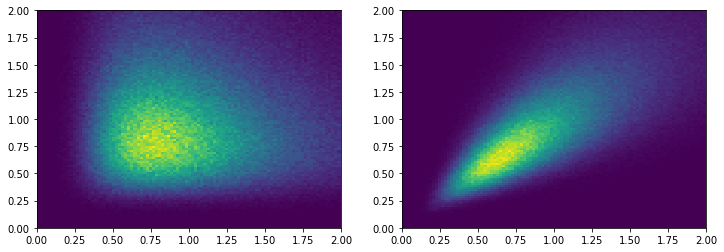
\includegraphics[width=0.9\linewidth]{figures/copula_lognormal.png}
\end{center}
\caption{Comparision of the joint 2D distributions in case of no correlation (left) and with a Gaussian correlation of 0.8 (right).}
\label{fig:joint_2d}
\end{figure}

In order to quantify the difference shown with the comparison of the two 2D plots we can calculate the probability that both companies default in the next six months.

So the probability that a single company default in six months regardless the other can be calculated from the \texttt{cdf} of the lognormal distribution.
Hence in case of independent probabilities what required is just the squared of this value (about 0.07\%).

\begin{ipython}
default_6m = lognorm(0.5).cdf(.5)
print(default_6m**2)
\end{ipython}
\begin{ioutput}
0.006860563560014724
\end{ioutput}

In the case of correlation instead we have to loop over the samples from the joint multivariate distribution (with correlation) and check how many times both values are less than \texttt{default\_6m}.

\begin{ipython}
success = 0.0
for i in range(samples):
    if max(x_corr[i]) < default_2:
        success += 1

print (success/samples)
\end{ipython}
\begin{ioutput}
0.044654
\end{ioutput}

This result can be interpreted graphically by saying that the entries in the "square" $[0, 0.5]$ in the left histogram are about 0.7\% of the total while the entries in the right plot in same "square" are about 4.5\% of the total. 
\end{solution}
